\chapter{Must Have Concepts}
During this chapter, we're going to discuss topics that help understand the technology developments made along the thesis project.

\section{The IOb-SoC Template}
\label{section:the_iob_soc_template}

\begin{figure}[!h]
    \centering
    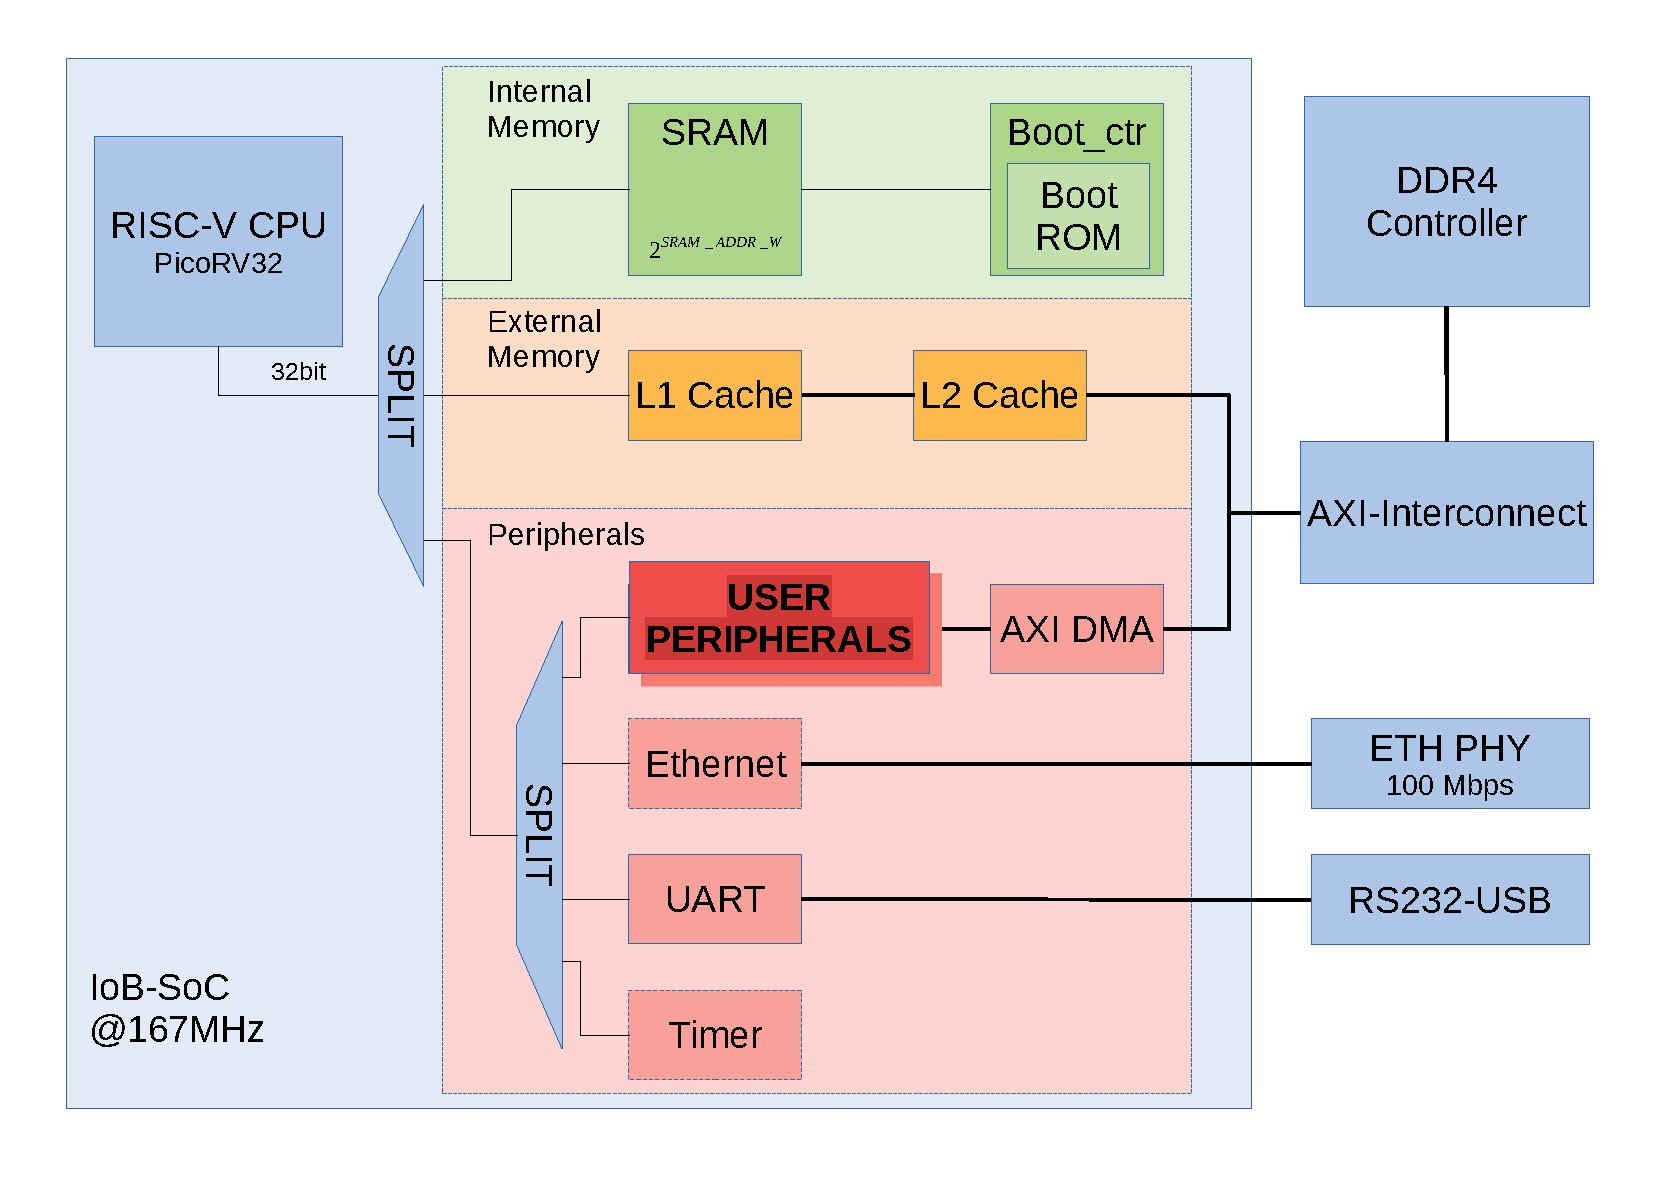
\includegraphics[width=0.7\linewidth]{bd_original.pdf}
    \caption{\textit{IOb-SoC} sketch.}
    \label{fig:bd_original}
\end{figure}

\subsection{Adding peripherals}
\subsection{Internal Buses}

\section{Open Source Verification tools}
For testing purposes, it is important to have a good hardware simulation environment. For that, we take advantage of already existing and well-developed tools. There exist a number of simulation tools, most of them are proprietary, as for example \textit{'xcelium'} from \textit{'Candence'}. Its utilization can increase the cost of a project significantly. In this Thesis we will make an effort of using open-source, free to use, verification tools. In specific, we will take advantage of \textit{'Icarus Verilog'} and \textit{'Verilator'}. Although both tools are for verification, they serve different purposes, due to their characteristics.

\begin{itemize}
    \item \textbf{\textit{'Icarus Verilog'}} is a Logic Simulator that uses verilog or system-verilog testbenchs to test the UUT (Unit Under Test). Unfortunately, its support for system-verilog is limited and some designs might not run in this simulator. \textit{'Icarus Verilog'} is also known as \textit{'IVerilog'}.
    
    After compiling the hardware design, \textit{'IVerilog'} outputs a file which can be run line by line to simulate designed logic.
    
    \item \textbf{\textit{'Verilator'}}
\end{itemize}

\textbf{The biggest differences} are: \textit{'Verilator'} only represents logic signal as 1's or 0's, contrary to \textit{'IVerilog'} which also represents unknown values as X's; Since \textit{'Verilator'} ends up being a C++ program it is much faster to run the simulation than with \textit{'IVerilog'}; On another perspective \textit{'Verilator'} is slower than \textit{'IVerilog'} to interpret the hardware logic design.
As such, it is easier to use \textit{'IVerilog'} to detect errors on the design, but it is better to use \textit{'Verilator'} for more complexed simulations.

\subsection{Qemu Simulation}
https://www.sifive.com/blog/risc-v-qemu-part-1-privileged-isa-hifive1-virtio

\section{RISC-V architecture}
The RISC-V \textbf{CLINT} is described
The RISC-V \textbf{PLIC} was first described in the privilege instructions documentation, but since version 1.10 it was moved to its own document.

\section{The Linux Boot Flow}
\subsection{Bootloader firmware}
\subsection{What is a device tree?}

\section{What is the UART16550?}


